%\stepcounter{subsection}
%\addcontentsline{toc}{subsection}{\protect\numberline{\thesubsection}<Monte Carlo Energy trends>}
The graphs in fig.~\ref{fig:UFtrends} show the Monte Carlo simulation results in terms of dispersive free energy and internal energy relative to SAFT at three different box sizes. Both sets of graphs show that a small box size has a higher energy than SAFT, while a larger box will have a lower energy than SAFT. This makes sense because as the box size increases longer wavelength fluctuations are allowed, and these longer wavelengths actually lower the allowed energy due to the decreased interactions in the low density regions being more than compensated by the increase in interactions in the high density regions. Given a constant box size, the high filling fraction simulations cannot fluctuate as much as the low filling fraction simulations, which explains the bulge in the two lower plots. The main point of the U,F trends plot is to show there is a transition where the simulations are over estimating the energy to under estimating the energy. This indicates the best box size should be somewhere between $L=5.66$ and $L=10.00"$.

These graphs inf fig.~\ref{fig:STCvtrends} show the Monte Carlo simulations results in terms of dispersive entropy and heat capacity per particle relative to SAFT at three different box sizes. It is interesting to see the entropy trends are nearly the inverse of the heat capacity trends. Both entropy and heat capacity require a derivative with respect to temperature, it is just that entropy is the negative derivative of Free energy while heat capacity is the positive derivative of internal energy. Given fig. \ref{fig:UFtrends} showed the internal and free energy spread out in a similar fashion as the temperature was increased, it isn't surprising entropy and heat capacity have inverse trends. Regarding the trend itself, the graphs suggest entropy of a small box will have more entropy than SAFT, while a large box will have a lower entropy than SAFT. This trend can be explained by the particles binding together in ways that SAFT could not take into account, and this extra binding will decrease the entropy simply because some configurations are now favored over other configurations. Just like the U,F trends, there is a transition between over and under estimating the entropy and heat capacity. This again indicates the best box size should be somewhere between $L=5.66$ and $L=10.00$.

Having verified the results from the simulations are as expected, the cost relative to SAFT is plotted in fig.~\ref{fig:Cost}. 
\pagebreak

\section{Trends in U,F}
\begin{figure}[h]
\vspace*{-40mm}
\hspace*{-6mm}
	\centering
	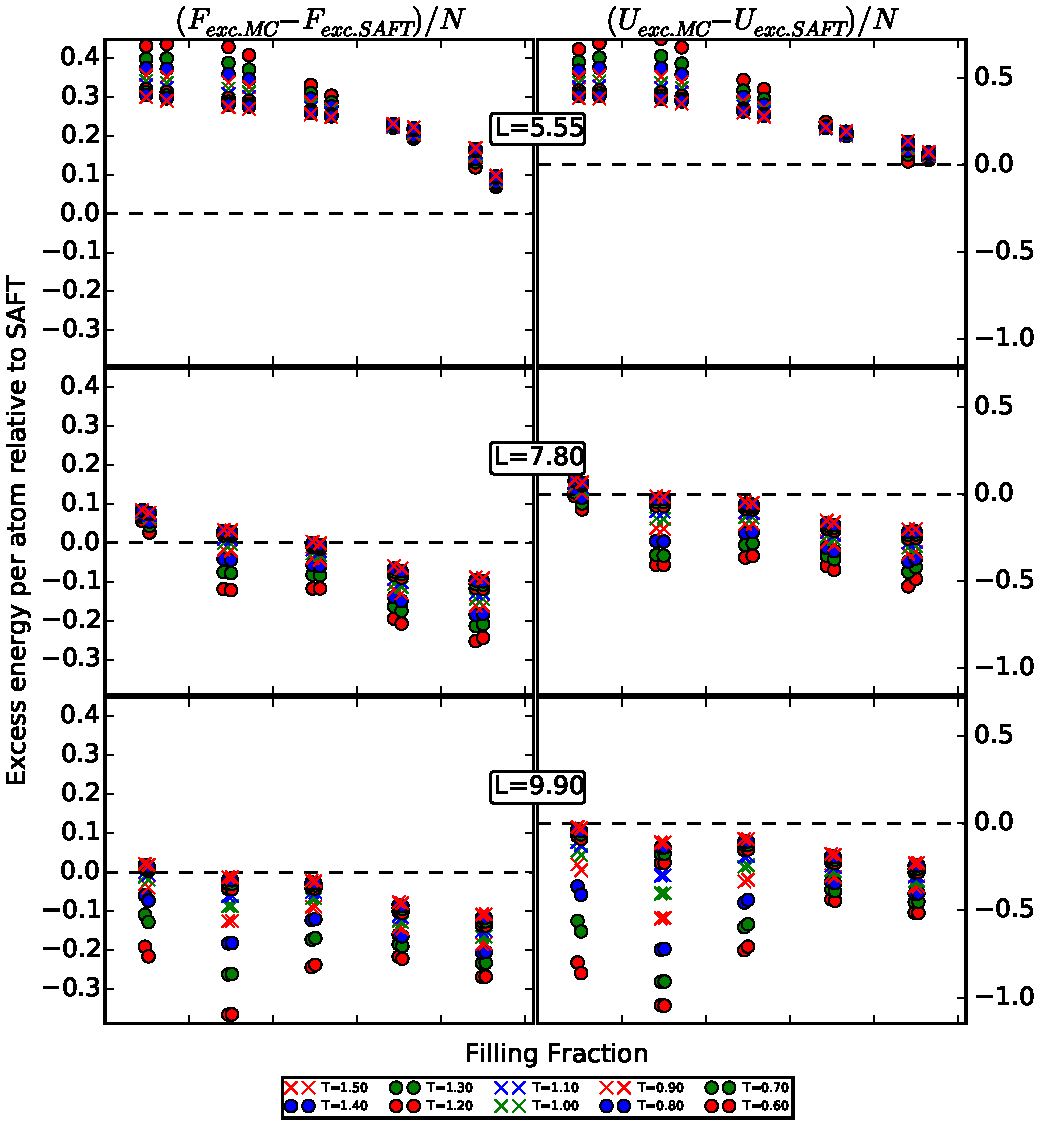
\includegraphics[scale=.9]{UFtrends-ww1.50.pdf}
	\caption{
	%\tiny	
	\scriptsize\textbf{
	}}
	\label{fig:UFtrends}
\end{figure}
%And also a citation example \cite{Forte2011}.
%And this one too \cite{Forte2013}


\pagebreak
\section{Trends in S,Cv}
\begin{figure}[h]
\vspace*{-40mm}
\hspace*{-6mm}
	\centering
	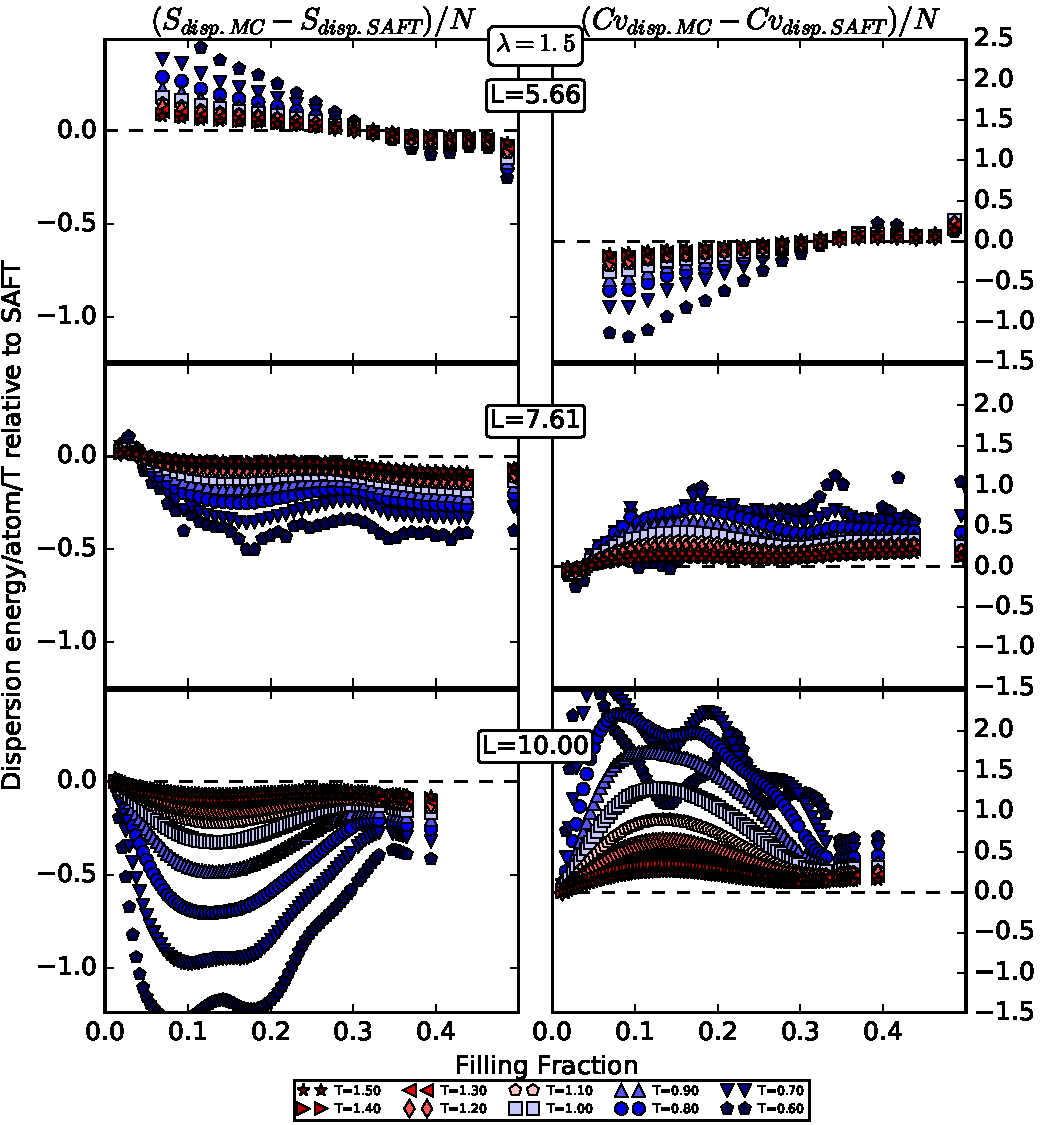
\includegraphics[scale=.9]{STCvtrends-ww1.50.pdf}
	\caption{\scriptsize\textbf{
	}}
	\label{fig:STCvtrends}
\end{figure}


\pagebreak
\section{Using Cost to Estimate Best Box Size}
\begin{figure}[h]
\vspace*{-10mm}
\hspace*{-6mm}
	\centering
	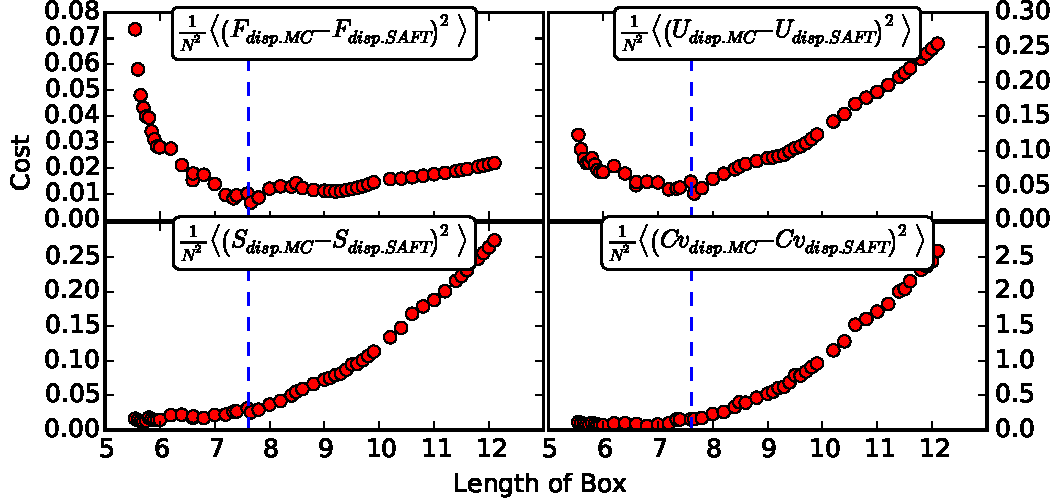
\includegraphics[scale=.9]{Costsmall-ww1.50.pdf}
	\caption{\scriptsize\textbf{
	These graphs show the cost function as a function of the box size for the dispersive free energy, internal energy, entropy, and heat capacity. The cost function is defiend as the mean square difference between the Monte Carlo simultions and SAFT evaulated at a filling fraction of [0.15,0.25,0.35,0.45] and evaluated for 0.6\textless T\textless 1.5. The dispersive free energy and internal energy show a minimum near L=7.6, while any box size less than L=8.0 seems to be just fine for the dispersive entropy and heat capacity.}}
	\label{fig:Cost}
\end{figure}
%\vspace*{-10mm}
\section{Coexistence: T vs Density}
\begin{figure}[h]
\vspace*{-10mm}
\hspace*{-6mm}
	\centering
	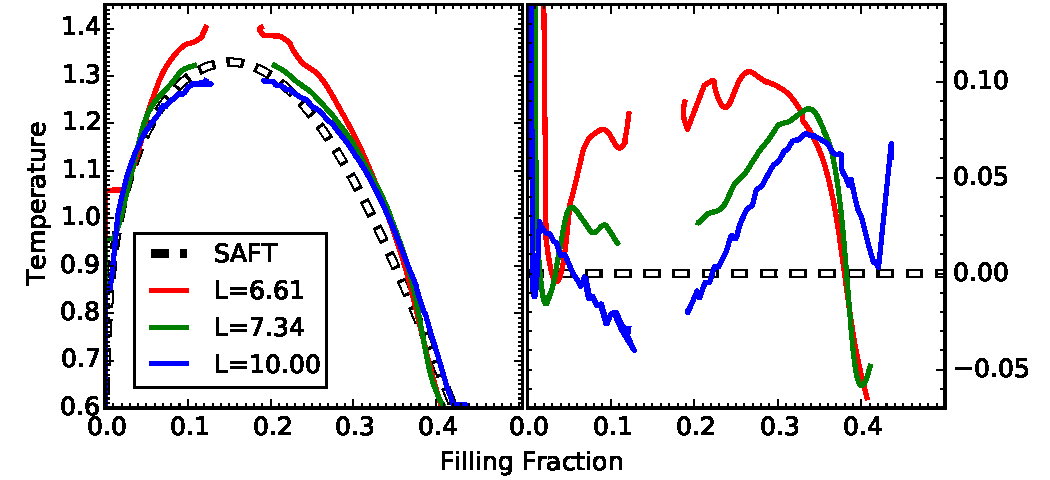
\includegraphics[scale=0.9]{coexistence-ww1.50.pdf}
	\caption{\scriptsize\textbf{
	Here the gas-liquid coexistence temperature as a function of filling fraction for three different Monte Carlo simulations are compared to SAFT. The box size L=6.61 clearly has a higher critical temperature than SAFT, while the box size L=10.0 clearly has a lower critical temperature than SAFT.}}
	\label{fig:Coexistence}
\end{figure}

\begin{figure}[h!]
\vspace*{-64.5mm}
\hspace*{-110mm}
	\centering
	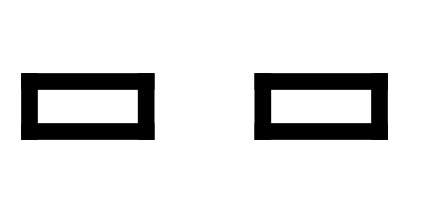
\includegraphics[scale=0.9]{coexistence-ww1.50BAR.png}
\end{figure}



